\documentclass[aps,reprint]{revtex4-1}
% Engine-specific settings
% Detect pdftex/xetex/luatex, and load appropriate font packages.
% This is inspired by the approach in the iftex package.
% pdftex:
\ifx\pdfmatch\undefined
\else
    \usepackage[T1]{fontenc}
    \usepackage[utf8]{inputenc}
\fi
% xetex:
\ifx\XeTeXinterchartoks\undefined
\else
    \usepackage{fontspec}
    \defaultfontfeatures{Ligatures=TeX}
\fi
% luatex:
\ifx\directlua\undefined
\else
    \usepackage{fontspec}
\fi
% End engine-specific settings
\usepackage[english]{babel}
\usepackage{csquotes}
% \usepackage[backend=biber, sortcites]{biblatex}
\usepackage{url}
\usepackage{textcomp}
\usepackage[usenames,dvipsnames,svgnames, table]{xcolor}
\usepackage[font={scriptsize}]{caption}
\usepackage{amsmath} \usepackage{amsthm} \usepackage{amsfonts}
\usepackage{amssymb}
\usepackage{enumerate}
\usepackage{tikz} \usepackage{float}
\usepackage[procnames]{listings}
\usepackage{pstool} \usepackage{pgfplots}
\usepackage{wrapfig} \usepackage{graphicx} \usepackage{epstopdf}
\usepackage{afterpage}
\usepackage{physics}
\usepackage{multirow}
\usepackage{gensymb}
\usepackage{algorithm}
\usepackage{microtype}
\usepackage[noend]{algpseudocode}
\usepackage{xcolor,colortbl}
\usepackage{microtype}
\usepackage{geometry}
\usepackage{hyperref}
\usepackage{graphicx}
\usepackage{caption}
\usepackage{subcaption}
\usepackage{lipsum}
% \usepackage{pythontex}
% \usepackage{authblk}
\usepackage{nth}
\usepackage{siunitx}
% \usepackage[toc,page]{appendix}
\floatstyle{plaintop}
\restylefloat{table}

% Custom commands
\newcommand{\unit}[1]{\:\mathrm{#1}}
\newcommand{\noref}[1]{\hyperref[#1]{\ref*{#1}}}
\newcommand{\nonref}[1]{\hyperref[]{\ref*{#1}}}
\newcommand\blankpage{%
  \null
  \thispagestyle{empty}%
  \addtocounter{page}{-1}%
  \newpage}

\newcommand{\mean}[1]{\langle #1 \rangle}

% Default fixed font does not support bold face
\DeclareFixedFont{\ttb}{T1}{txtt}{bx}{n}{7} % for bold
\DeclareFixedFont{\ttm}{T1}{txtt}{m}{n}{7}  % for normal

\newcommand\numberthis{\addtocounter{equation}{1}\tag{\theequation}}
\DeclareCaptionFont{white}{\color{white}}
\DeclareCaptionFormat{listing}{\colorbox{gray}{\parbox{\columnwidth}{#1#2#3}}}
\pgfplotsset{compat=1.14} %TODO: Setting this removed several error messages, should it be here!?


% Biber for references
% \bibliographystyle{aipauth4-1}

\begin{document}
\sisetup{detect-all}
\title{Ising (Or should I say Ezing?)}
\author{Erlend Lima}
\thanks{All code related to or referred by this paper was written in
  collaboration with Frederik J. Mellbye. This paper itself is written by
 solely the author.}
\affiliation{University of Oslo, Oslo, Norway \\ Source code available at: \url{https://github.com/Caronthir/FYS3150/tree/master/Project4}}
\date{\today}

\begin{abstract}
Once again the abstract abstractifies the abstractness of the abstract mathematical
equations than govern the universe.
\end{abstract}
\maketitle
\tableofcontents
\makeatletter
\let\toc@pre\relax
\let\toc@post\relax
\makeatother

\newpage

\section{Introduction}
\label{sec:introduction}

In his 1924 PhD thesis, Ernt Ising 
solved the one dimensional Ising model devised by his adviser, Wilhelm
Lenz~\cite{weicai}. Ising showed that no phase transition can occur in one
dimension, and so triumphantly declared that no phase transition can occur in
any dimension. Lars Onsager proved otherwise when he showed that there indeed
were phase transitions in two dimensions. Even though Ising was wrong, his name
is amongst the most common names in statistical mechanics. 
\section{Theory}
\label{sec:theory}

\subsection{The Ising Model}
\label{sec:isingmodel}

The Ising model is a microcanonical model which describes a lattice of discrete spins taking binary values, where each
spin interacts with its neighbors. Although simple, the Ising model is capable of modeling real
world phenomena such as ferromagnetism and phase transitions.

A lattice \(\Lambda\) is a \(d\)-dimensional graph with the nodes \(k\in\Lambda\) being spins
taking a discrete binary value, \(s_{k}\in\{-1, 1\}\). As the lattice is often
finite, its boundaries needs to be taken into account. These are treated as
periodic boundaries, where the edge on the left is connected to the edge on the
right, and the top to the bottom. For a one dimensional lattice, this topologically equivalent
to a string, while a two dimensional lattice is topologically equivalent to a torus.

For a lattice of \(N\) nodes, its energy is

\begin{equation}
  \label{eq:2}
 E = -\sum_{<kl>}^{N}J_{k,l}s_{k}s_{l} - \sum_{k}^{N}\mathcal{B}_{k}s_{k}
\end{equation}

where \(<kl>\) denotes that the sum is taken over the neighboring spins.
Between any two spins \(k, l \in \Lambda\) there is an interaction \(J_{k,l}\),
and for any spin there is the possibility of an external magnetic field with
interaction \(\mathcal{B}_{k}\). Assuming that the spin interactions are equal
for all spins and the absence of an external magnetic field, the energy
simplifies to

\begin{equation}
  \label{eq:3}
  E = -J\sum_{<kl>}^{N}s_{k}s_{l}
\end{equation}

For \(J>0\), it is favorable for neighboring spins to align, causing the
creation of magnetic domains throughout the lattice~\cite{physicslectures}.
This is called ferromagnetism. For \(J<0\), it is more favorable for spins to
point in opposite direction. The physical interpretation of this is
paramagnetism. In the remainder of this paper, it is assumed that \(J>0\).
The magnetism of the system is simply is sum over the spins,
\begin{equation}
  \label{eq:1}
  \mathcal{M} = \sum_{k} s_{k}
\end{equation}

Being microcanonical, the Ising model can be described by Boltzmann statistics.
Using this fact, it can be shown~\cite{physicslectures} that the heat capacity is
\begin{equation}
  \label{eq:4}
  C_V = \frac{\mean{E^2} - \mean{E}^2}{kT^2}
\end{equation}
and that the magnetic susceptibility is
\begin{equation}
  \label{eq:5}
  \chi = \frac{\mean{\mathcal{M}^2} - \mean{\mathcal{M}}^2}{kT}
\end{equation}
In addition, the first moment of energy can be written as
\begin{equation}
  \label{eq:6}
  \mean{E} = - \pdv{\ln{Z}}{\beta}
\end{equation}

\subsection{Phase Transitions of the Two Dimensional Ising Model}
\label{sec:phase-trans-two}
The Ising model in two dimensions without an external magnetic field was first
solved by Lars Onsager. He showed that there exists a phase transition for some
critical temperature \(T_{C}\), in contrast to the one dimensional case. Ad this
temperature, the spins rapidly flip, causing spikes in thermodynamic quantities such as
heat capacity. The quantities can be modeled as~\cite{project3}


\begin{align*}
  \mean{M(T)} &\sim (T - T_C)^\beta \\
  C_V(T) &\sim |T_C - T|^\gamma \\
  \chi (T) &\sim |T_C - T|^{-\alpha}
\end{align*}
where $\alpha = 0$, $\beta = 1/8$ and $\gamma = 7/4$ are critical exponents.

\subsection{Analytic Solution}
\label{sec:analytic-solution-}

For a two dimensional lattice with the above assumptions, namely the absence of a magnetic field, \(J>0\),
periodic boundaries and with a lattice size of \(L=2\) for a total of \(4\)
spins, analytical expressions for thermodynamic quantities can be found.
Labeling each spin \(s_{1}\) through \(s_{4}\), a possible spin configuration is
shown in figure~\ref{fig:22lattice}. There are \(2^{4}=16\) unique microstates, one
of which is shown in the figure. However, because of the periodic boundaries,
many of the spin states are isomorphic to each other, resulting in only five
distinct macrostates. For example, the two spin configurations in the figure are
ismorphic, as one can simply interchange the rows (or, if you will, pull the
entire lattice down through the periodic boundary) and then relabel the spins. A
complete summary is shown in table~\ref{tab:2x2values}.

\begin{figure}[H]
  \centering
  \begin{tikzpicture}[thick]
    \draw[->] (0,0) -- (0,.3)  node [label=left:{$s_1$}] {};
    \draw[->] (1,0) -- (1,.3)  node [label=right:{$s_2$}] {};
    \draw[<-] (0,1) -- (0,1.3) node [label=left:{$s_3$}] {};
    \draw[<-] (1,1) -- (1,1.3) node [label=right:{$s_4$}] {};
    \draw[-] (-.75,-.4) rectangle (1.75,1.9);

    \draw[<-] (3,0) -- (3,.3)  node [label=left:{$s_1$}] {};
    \draw[<-] (4,0) -- (4,.3)  node [label=right:{$s_2$}] {};
    \draw[->] (3,1) -- (3,1.3) node [label=left:{$s_3$}] {};
    \draw[->] (4,1) -- (4,1.3) node [label=right:{$s_4$}] {};
    \draw[-] (2.25,-.4) rectangle (4.75,1.9);
  \end{tikzpicture}
  \caption{$2 \times 2$ enumerated lattice showing two different microstates
    corresponding to the same macrostate.}
  \label{fig:22lattice}
\end{figure}


\begin{table}[H]
  \caption{Possible states and associated energies, magnetizations and degeneracies.
  The same table is also found in \cite{mortenjensen}}
  \label{tab:2x2values}
    \begin{tabular}{cccc}
      Spins up & Energy [$J$] & Magnetization & Multiplicity \\\hline
      4        & -8           & 4             & 1            \\
      3        & 0            & 2             & 4            \\
      2        & 0            & 0             & 4            \\
      2        & 8            & 0             & 2            \\
      1        & 0            & -2            & 4            \\
      0        & -8           & 4             & 1
    \end{tabular}
\end{table}

Armed with the complete knowledge of the macro states, it is feasible to compute
the partition function,

\begin{align*} \label{eq:partitionfunc}
  Z &= \sum_k e^{\beta E_k}\\
    &= 2 e^{8\beta J} + 2 e^{- 8\beta J} + 12\\
  &= 4 \cosh{(8\beta J)} + 12
\end{align*}
where \(\beta = 1/kT\) and~\eqref{eq:3} was used.


The mean energy (energy expectation value) is given by
\begin{align*}
  \mean{E} = -\frac{8 J \sinh{(8\beta J)}}{\cosh{(8\beta J)} + 3}
\end{align*}
and the mean of the square of the energy is given by
\begin{align*}
  \mean{E^2} = \frac{256 J^2 \cosh{(8\beta J)}}{4\cosh{8\beta J} + 12}.
\end{align*}
The energy expressions can be used to compute the heat capacity $C_V$, which
is given by
\begin{align*}
  C_V = \frac{1}{kT} \left( \mean{E^2} - \mean{E}^2 \right)
\end{align*}

Similarly, the magnetization properties are given by
\begin{align*}
  \mean{M} &= 0 \\
  \mean{M^2} &= \frac{8e^{8 J \beta} + 8}{\cosh{8\beta J} + 3}
\end{align*}
which can be used to find the susceptibility using equation ~\ref{eq:sus}.

\subsection{Numerical Solution}
\label{sec:numerical-solution}

Simple systems such as the \(2\times 2\) case considered in the
previous sections lend themselves to analytical solutions, but as the systems
grow larger, it becomes increasingly difficult to find an expression for the
partition function. Instead, such systems can be solved numerically by
sidestepping the partition function completely.

This is done using Monte Carlo simulations, often through the
Metropolis-Hastings algorithm. See~\cite{physicslectures} for a detailed
explanation. A rough outline of the method is given as

\begin{enumerate}
  \item Select randomly $L^2$ spins from the \(L\times L\) lattice.
  \item Calculate the change in energy $\Delta E$ of the entire system if a randomly selected spin was to
  be flipped.
  \item Draw a random number from the uniform distribution, and compare
  \begin{align*}
    U(0,1) \leq e^{-\beta \Delta E}.
  \end{align*}
  If this is true, the spin is flipped. If this evaluates as false, do not flip
  the spin. If $\Delta E < 0$ the spin is flipped regardless, to model that physical
  systems usually tend to lower energy configurations.
\end{enumerate}

As long as the temperature is sufficiently low, the system will decrease in
energy until an equilibrium state as been reached.

Since the lattice is discrete, possible values for the change in energy \(\Delta
E\) is finite. As each flip only impacts the spin's neighbors, there are in fact
only five possible values for \(\Delta E\). It can be shown~\cite{physicslectures}
that these values are

\begin{equation*}
  \Delta E = \{-8J,\: -4J,\: 0,\: 4J,\: 8J\}
\end{equation*}

Precomputation of these values speeds up the algorithm by a noticeable amount.

\section{Method}
\label{sec:method}

\subsection{Overview}
\label{sec:overview}


The goal was to solve the Ising model numerically using the Metropolis-Hastings
algorithm as outlined in~\ref{sec:numerical-solution}. This was done completely
in C++ and partially in Julia, both producing data which was analyzed using
Python. The model was made highly flexible and user friendly, where the user could
type the parameters into a JSON-file which the C++ solver would read and solve
the corresponding model.
The Python script could then analyze the data without any need to specify the
resulting files nor their format - the script figured out this automatically.
For a more in-depth explanation of the workflow and the source code, see the
GitHub repository.

\subsection{Boundary Conditions}
\label{sec:boundary-conditions}

The boundary conditions 
\section{Results}
\label{sec:results}

\begin{figure}[H]
  \centering
  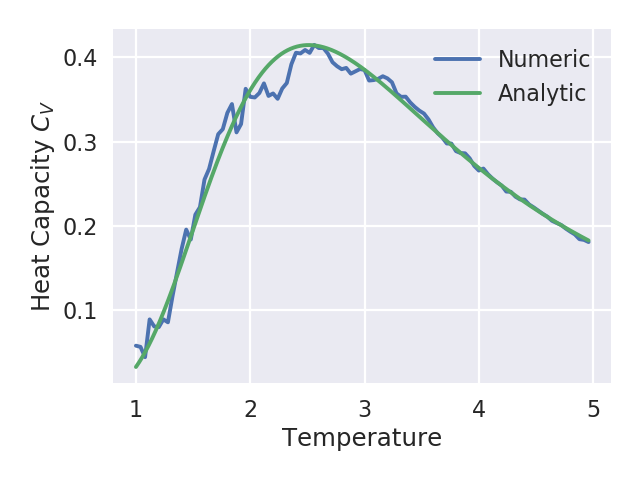
\includegraphics[width=\columnwidth]{figures/L2Ne4.png}
  \caption{$2 \times 2$ lattice with $M = 10^4$ MC iterations.}
  \label{fig:L2Ne4}
\end{figure}
\begin{figure}[H]
  \centering
  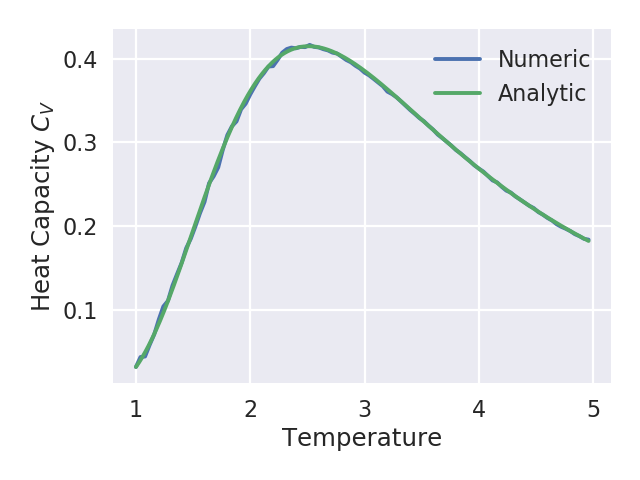
\includegraphics[width=\columnwidth]{figures/L2Ne5.png}
  \caption{$2 \times 2$ lattice with $M = 10^5$ MC iterations.}
  \label{fig:L2Ne5}
\end{figure}
\begin{figure}[H]
  \centering
  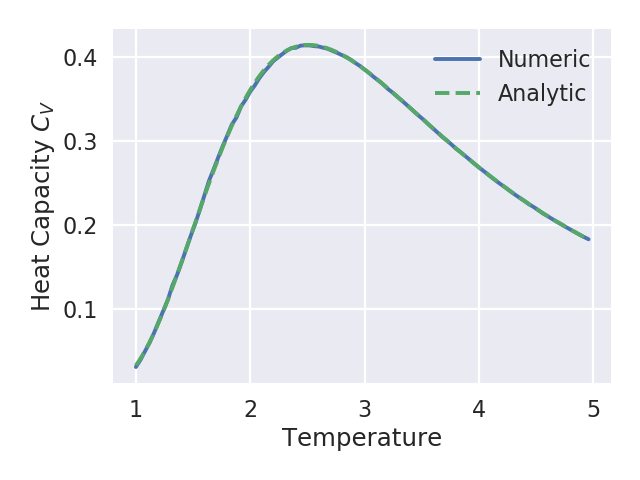
\includegraphics[width=\columnwidth]{figures/L2Ne6.png}
  \caption{$2 \times 2$ lattice with $M = 10^6$ MC iterations.}
  \label{fig:L2Ne6}
\end{figure}
\begin{figure}[H]
  \centering
  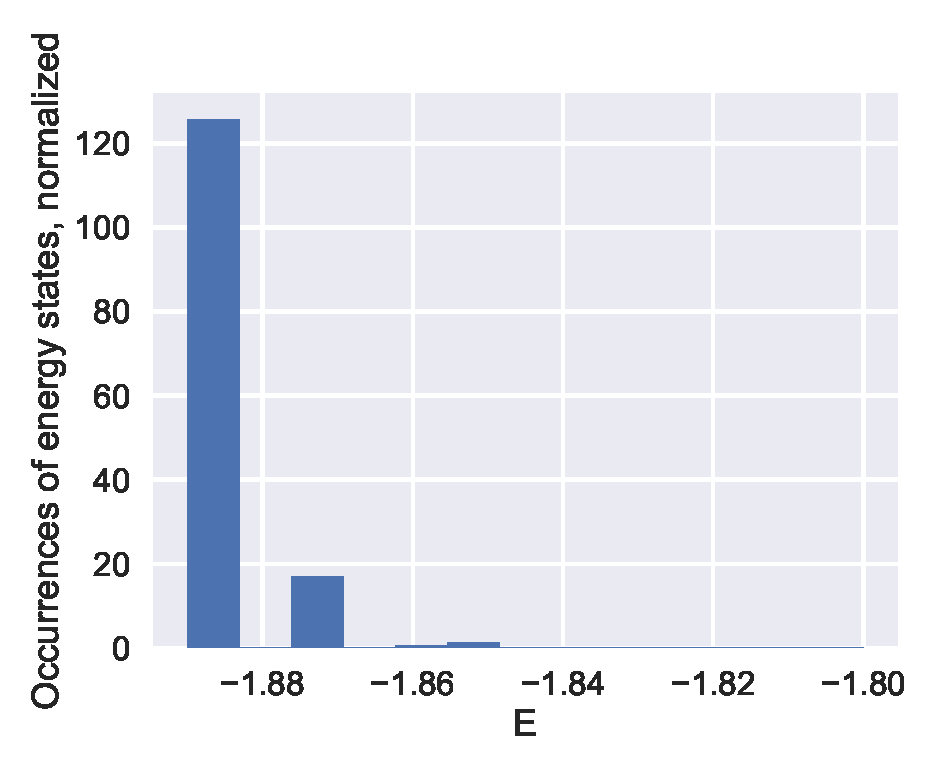
\includegraphics[width=\columnwidth]{figures/4da.eps}
  \caption{\label{fig:4da} Histogram over the energy states with \(T=1.0\) kT/J.
  The variance is \(\sigma^{2} \approx 5.845\cdot 10^{-5}\)}
\end{figure}

\begin{figure}[H]
  \centering
  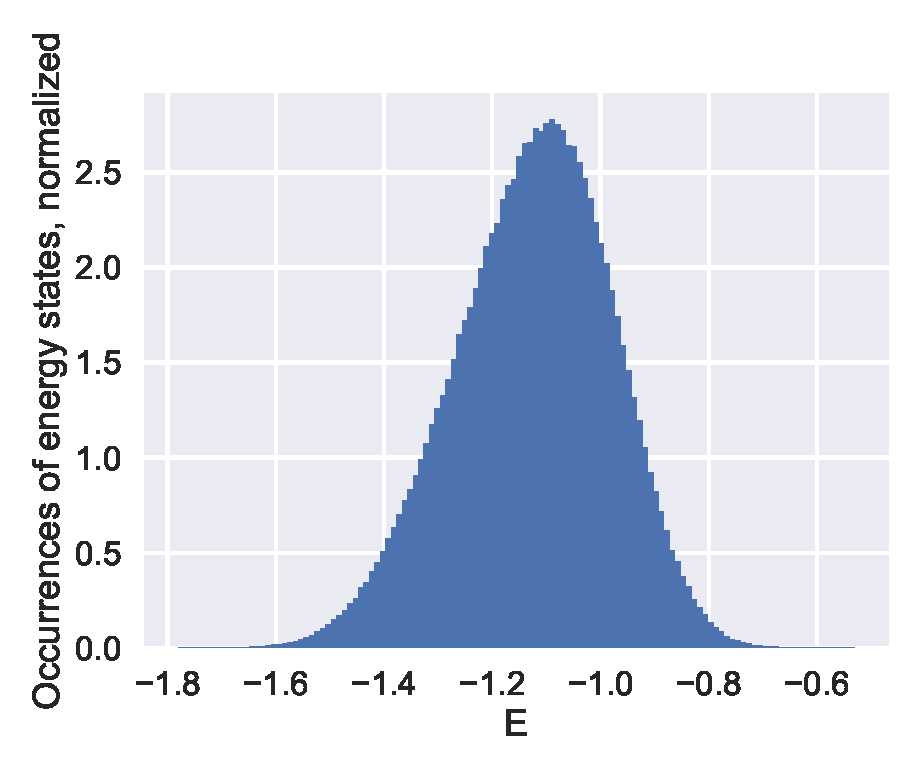
\includegraphics[width=\columnwidth]{figures/4db.eps}
  \caption{\label{fig:4db} Histogram over the energy states with \(T=2.4\) kT/J.
  The variance is \(\sigma^{2} \approx 0.0203\)}
\end{figure}

\begin{figure}[H]
  \centering
  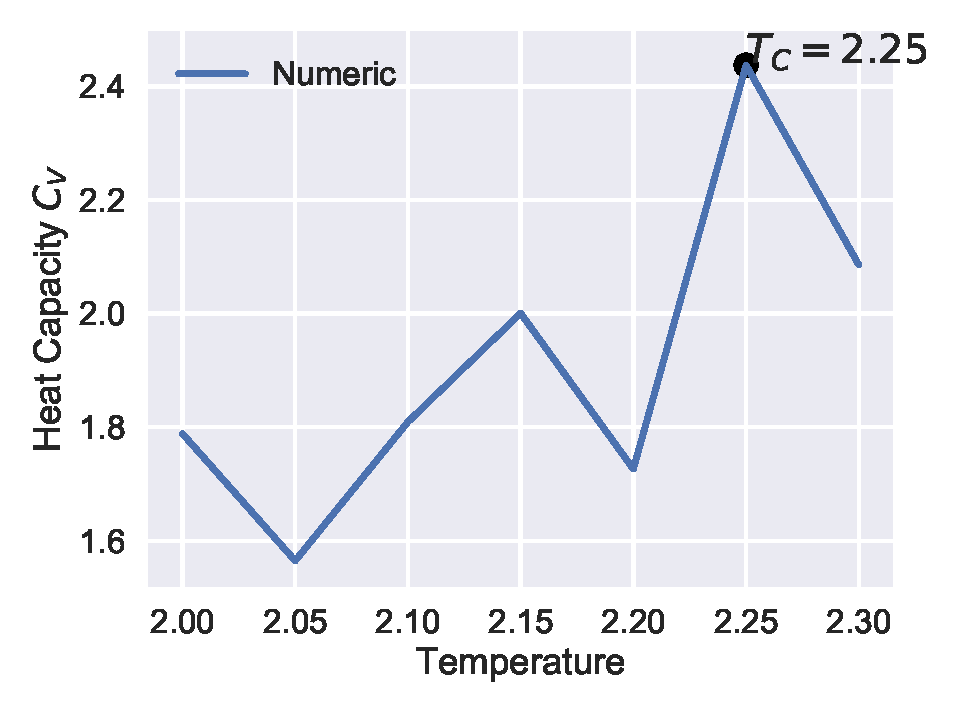
\includegraphics[width=\columnwidth]{figures/L100Cv.eps}
  \caption{\label{fig:100CVTc} Heat capacity for \(L=100\).}
\end{figure}

\begin{figure}[H]
  \centering
  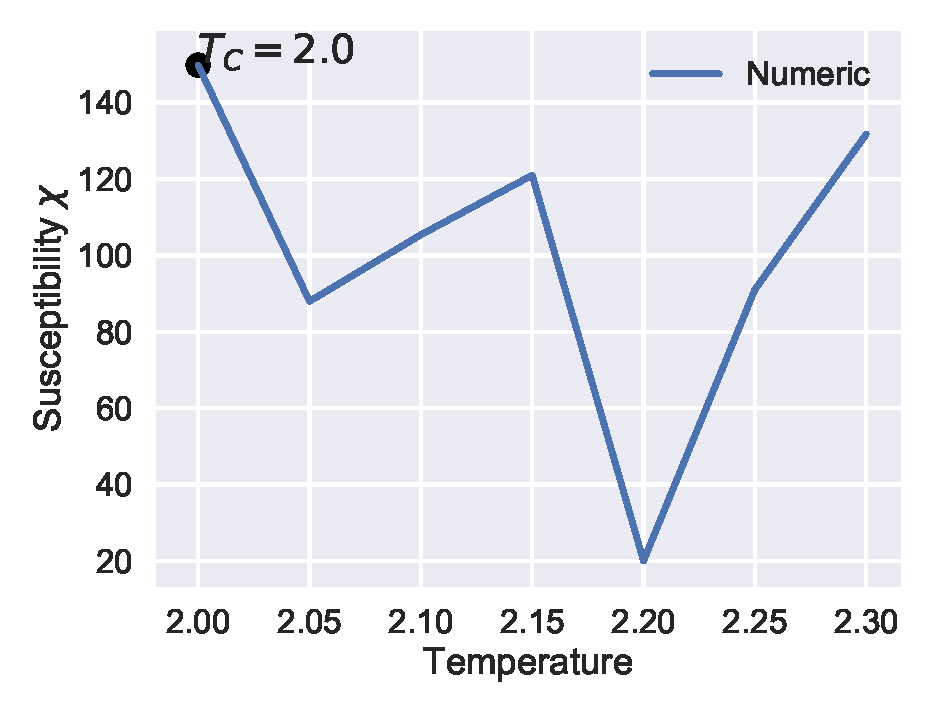
\includegraphics[width=\columnwidth]{figures/L100sus.eps}
  \caption{\label{fig:100CVTc} Magnetic susceptibility for \(L=100\).}
\end{figure}
\section{Discussion}
\label{sec:discussion}

\section{Conclusion}
\label{sec:conclusion}

\bibliography{references}
\blankpage
\appendix
\section{Appending appendices is easy with the appendix package.}
\blankpage
\end{document}

% Local Variables:
% TeX-engine: luatex
% End:
